% NOTE TO AIP TYPSETERS: TO CONVERT FROM TWO-COL TO PREPRINT, SWITCH
% COMMENTOUT COMMAND FROM A TO B IE. USE:
%
%%\documentclass[prl,twocolumn,showpacs,twocolumngrid,superbib]{revtex4}
%\documentclass[prl,twocolumn,twocolumngrid,superbib]{revtex4}
%\newcommand{\commentoutB}[1]{}
%\newcommand{\commentoutA}[1]{#1}
%
% INSTEAD OF THE FOLLOWING:
%
\newcommand{\commentoutB}[1]{#1}
\newcommand{\commentoutA}[1]{}
%\documentclass[prl,aps,preprint,showpacs,superbib]{revtex4}
\documentclass[prl,aps,preprint,superbib,12pt]{revtex4}

\usepackage{graphicx}
\usepackage{amsfonts}
\usepackage{amsmath}
\usepackage{bm}
\usepackage{alltt}
\usepackage{fancyhdr}
\newcommand{\bms}[1]{{\boldsymbol #1}}
\renewcommand{\thefootnote}{\fnsymbol{footnote}}

%\draft
%\tighten
\pagestyle{fancy}

\begin{document}

\title{Geometry Optimization of Crystals by the Quasi-\\
       Independent Curvilinear Coordinate Approximation}

\author{K\'aroly N\'emeth\footnotemark[1]}
\author{Matt Challacombe}

\affiliation{Theoretical Division,\\ Los Alamos National Laboratory, \\ Los Alamos, NM 87545, USA}

\date{\today}

\begin{abstract}
This paper presents a performance-assessment 
of the recently developed quasi-independent curvilinear coordinate
approximation (QUICCA) method [K. N\'emeth and M. Challacombe,
J. Chem. Phys. {\bf 121}, 2877, (2004)] for the optimization of crystal 
structures. 
We demonstrate that the concept of quasi-independent
curvilinear coordinates is valid also under periodic boundary 
conditions,
and it leads to highly efficient crystal structure optimizations
as illustrated by a series of test calculations. 
The asessment of QUICCA for the optimization of crystal structures
prooves that QUICCA is a generally applicable algorithm
that is highly efficient for the optimization of both isolated 
molecules and crystals while it preserves an unparalleled robustness 
and simplicity of implementation.
\end{abstract}

%\pacs{31.15.-p,31.15.Ne,02.60.Pn, 45.10.Db, 02.40.Hw} 

\maketitle

\footnotetext[1]{\tt KNemeth@LANL.Gov}

\section{Introduction}
Internal coordinates based on chemical intuition 
are now routinely used in the optimization of 
molecular structures by most standard quantum chemistry program 
packages. Internal coordinates are more advantageous 
for geometry optimization since they exhibit much less 
harmonic and anharmonic vibrational coupling then Cartesians do
\cite{PPulay69,GFogarasi79,GFogarasi92,PPulay77}.
The reduced vibrational coupling allows for much larger steps during the
optimization and results in at least 7-10 times smaller number of 
of optimization steps on small and medium sized molecules
as compared to Cartesian conjugate gradient schemes \cite{TBucko05}.  

Until recently, internal coordinates have been used only to optimize
the structure of isolated molecules.
In recent articles by Kudin {\it et.al.} \cite{KKudin01} and by
Andzelm {\it et.al.} \cite{JAndzelm01} crystal structure optimizations
have been carried out in internal coordinates.
These authors proposed a way
how to build Wilson's B matrix \cite{EWilson55} 
when periodic boundary conditions are present. 
The scheme presented by Kudin {\it et.al.} \cite{KKudin01} allowed for 
the simultaneous relaxation of atomic positions and lattice parameters,
while the one by Andzelm {\it et.al.} \cite{JAndzelm01}  concerned only 
with the relaxation of atomic positions while lattice parameters have 
been fixed. 
An important improvement in the construction of the B-matrix
was very recently carried out by Bu\v{c}ko, Hafner and {\'A}ngy{\'a}n
\cite{TBucko05}.
These authors realized that 
all internal coordinates may have non-vanishing contribution
to the displacement of lattice parameters, and not only those
that cross the boundaries of the central cell. 
In our opinion, the paper of Bu\v{c}ko, Hafner and {\'A}ngy{\'a}n
provides the first complete determination of Wilson's B matrix
for crystals. This definition of the B matrix will be used through
the present paper. 

In the present article we want to assess the performance of our recently
developed optimization algorithm, the Quasi Independent Curvilinear 
Coordinate Approach (QUICCA) \cite{KNemeth04} 
in crystal structure environment.
QUICCA is based on a radical exploitation of the approximate decoupling
of internal coordinate motions within a molecule and is very simple 
to implement, robust and very efficient for isolated molecules while
its computational cost scales linearly with the system-size for each 
optimization step. However, nothing is known yet about the 
applicability of QUICCA for crystals. In crystals, coupling effects
may be very different from the ones in isolated molecules. If QUICCA
works similarly well for crystals as it does for isolated molecules
it can be used as a generally applicable, extremely robust 
internal coordinate optimizer for the optimization of large 
molecules and crystals. 

In the following, we first review the construction of Wilson's B matrix
for crystals (Sec. \ref{crystalBmat}), then the QUICCA algorithm is 
reviewed as applied for crystals (Sec. \ref{QUICCAreview}, 
finally results of test calculations
ranging over a broad class of crystalline systems are presented
(Sec. \ref{ResDissc}). Finally, we conclude the analysis of the results
in that QUICCA is a very efficient method for optimizing both
crystal structures and isolated molecules (Sec. \ref{Conclusions}).

\section{Methodology}
\subsection{Wilson's B matrix for crystals}
In this section we briefly review how the elements of Wilson's
B matrix can be calculated for crystals. A more detailed discussion 
of this issue can be found in Ref. \onlinecite{TBucko05}.

The independent geometrical variables of a crystal are the 
fractional coordinates, $f_{k}$ and the lattice vectors, $h_{l}$.
The absolute Cartesian position, $r_{k}$ of the $k$-th atom
can be decomposed as a funtion of both the fractional coordinates 
$f_{k}$ of atom $k$ and the lattice vectors:
\begin{equation}
r_{i} = h f_{i} ,
\end{equation}
where the matrix $h$ contains the Cartesian components of the 
$h_{1}$, $h_{2}$ and $h_{3}$ lattice vectors in its 
columns, respectively.

The B matrix for crystals contains the total derivatives 
of internal coordinates with respect to fractional ones
and lattice vectors:
\begin{equation}
B_{ik} = \frac{d \phi_{i}}{d f_{k}} ,
\end{equation}
\begin{equation}
B_{il} = \frac{d \phi_{i}}{d h_{l}} ,
\end{equation}
where $\phi_{i}$ is the $i$-th internal coordinate,
and $B_{ik}$ is a 3-component vector, similar to $f_{k}$ and $h_{l}$.

In order to compute elements of the B matrix of a crystal, the above
expressions must be
related to B matrix elements of isolated molecules. This decomposition
can be done by the application of the chain rule to the above 
total derivatives, which results in
\begin{equation}
B_{ik} =  \frac{\partial \phi_{i}}{\partial r_{k}} h ,
\end{equation}
and 
\begin{equation} \label{Blattice}
B_{il} =  \sum_{m=1}^{4} 
          \frac{\partial \phi_{i}}{\partial r_{m}} f_{ml},
\end{equation}
where $\frac{\partial \phi_{i}}{\partial r_{k}}$ and 
$\frac{\partial \phi_{i}}{\partial r_{m}}$ are row-vectors and contain
the partial derivative of the $i$-th internal coordinate
with respect of the absolute Cartesian positions of 
the $k$-th and $m$-th atoms. $f_{ml}$ represents the
$l$-th component of the fractional coordinates of the $m$-th atom.
These partial derivatives are identical
with the B matrix elements of isolated molecules. The summation
in Eq. \ref{Blattice} goes over all atoms that compose $\phi_{i}$,
i.e. in case of primitive internal coordinates over maximum $4$ atoms. 

\subsection{Preparation of gradients}
Our linear scaling electronic structure program, MondoSCF \cite{MondoSCF} provides
the energy gradients on the absolute Cartesian positions, 
$\frac{\partial E}{\partial r_{k}}$, and the total derivatives
of the energy with respect to lattice vector components, 
$\frac{d E}{d h_{l}}$.
To calculate the forces, $\frac{d E}{d \phi_{i}}$, which act on the
internal coordinates, the total derivatives of the energy,
$\frac{d E}{d f_{k}}$ and 
$\frac{d E}{d h_{l}}$ are needed of which $\frac{d E}{d h_{l}}$ is 
given by our electronic stucture code.
$\frac{d E}{d f_{k}}$ can easily be calculated as:
\begin{equation}
\frac{d E}{d f_{k}} = \frac{\partial E}{\partial r_{k}} h .
\end{equation}
For the sake of completeness the relationship between total and
partial derivatives of the energy with respect of the lattice vectors
is defined by    
\begin{equation}
\frac{d E}{d h_{l}} = \frac{\partial E}{\partial h_{l}} +
                      \sum_{n=1}^{N_{a}} 
                      \frac{\partial E}{\partial r_{n}} f_{nl} ,
\end{equation}
where $N_{a}$ is the number of atoms in the elementary cell.



\subsection{Coordinate transformations}
Once the B matrix is given, the gradients on the internal coordinates
are calculated by solving 
\begin{equation} \label{solveintcgrads}
B^{t} g_{i} = g_{c} ,
\end{equation}
where the first $3N_{a}$ elements of $g_{c}$ contain 
the $\frac{d E}{d f_{k}}$ gradients and the last $9$ elements contain
the $\frac{d E}{d h_{l}}$ ones and the superscript $t$ means 
transposition.

The coordinate transformations are carried out in a linear scaling 
fashion, as described in Refs. \onlinecite{KNemeth00} and 
\onlinecite{KNemeth01}. It is worth to mention, that the last 9 columns
of the B matrix which refer to lattice derivatives of the internal 
coordinates may be full, as opposed to the first $3N_{a}$ columns 
which are extremely sparse. Even with 9 colums full, the Cholesky
factorization of the $G_{c}=B^{t}B$ matrices can be carried out
in a linear scaling fashion, since the first $3N_{a} \times 3N_{a}$
block of $G_{c}$ preserves its extreme sparsity, similar to the
case of isolated molecules \cite{KNemeth00}.
Thus the solution of Eq. \ref{solveintcgrads} can be carried out 
in a linear scaling fashion also for crystals.
Note that the sparsity in the Cholesky factorization step cannot be
preserved when an alternative solver, based on the $G_{i}=BB^{t}$
matrix is used, thus this latter route is inefficient to carry out
the coordinate transformation for large crystals.

Once predictions are done for improved values of internal coordinates
on the basis of internal coordinate gradients and the QUICCA 
\cite{KNemeth04} algorithm, the new Cartesian coordinates 
are calculated via the iterative back-transformation
as described in Ref. \onlinecite{KNemeth04}, which also scales 
linearly with the system-size. At each step of the iterative 
back-transformation fractional coordinates and lattice vectors
are updated and the corresponding atomic Cartesian coordinates are
generated to determine the updated values of internal coordinates
at an updated crystal structure. The rest of the back-transformation
is the same as what is used for isolated molecules.

\subsection{The QUICCA algorithm for crystals}
Details of the QUICCA algorithm for geometry optimization 
of isolated molecules are 
described in our previous paper \cite{KNemeth04}. Here we provide 
only a very brief summary of the most important features of the 
optimizer.
QUICCA is based on the realization of the fact, that internal coordinate
gradients show trends during geometry optimization.
These trends can be formalized by weighted curve fitting for each 
individual internal coordinate, over internal coordinate value and 
gradient pairs.
In practice, this curve fitting is most robust with just a line-fit. 
The root of the
fitted curve (line) provides an improved estimate for the minimum
along the internal coordinate. Collectively, these minima determine
the optimization step at the actual geometry.
QUICCA works well, because internal coordinates exhibit  
reduced harmonic and anharmonic vibrational coupling, as
compared to Cartesian ones. Furthermore, the fitting process
has an important averaging effect on the vibrational coupling
that also strongly contributes to the success of QUICCA.
A typical fitting process of a gradient curve is illustrated in 
Fig. \ref{iceIh} on a hydrogen bond of the icosahedral (P63/MMC)
ice structure \cite{AGoto90}.

\begin{figure}[h]
\resizebox*{3.5in}{!}{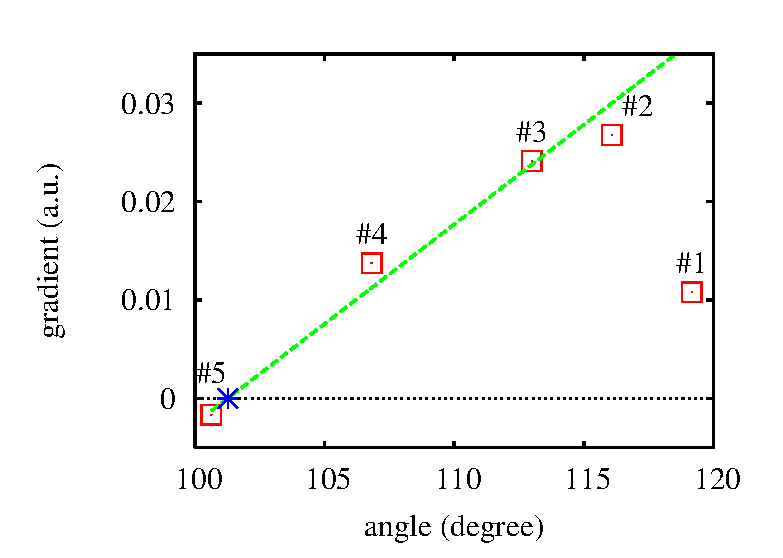
\includegraphics{IceIhfit.eps}}
\caption{
Progression of gradients on a hydrogen bond coordinate
of the icosahedral ice crystal.
Energies and forces have been obtained by the Hartree-Fock
model in STO-3G basis set.
The optimization was started from the crystallographic structure
\cite{AGoto90}.
The numbers in the picture
indicate the sequence of optimization steps. The dashed line represents
a linear fit, the star the predicted location of the minimum.}
\label{iceIh}
\end{figure}


\section{Implementation}

\subsection{Data preparation}
During the process of geometry optimization atomic positions
of the central cell may be folded back to the opposite side of the 
cell, for varios reasons, e.g. because the folded coordinates 
are more convenient for energy and gradient evaluation. The folded
atoms will be translated by a lattice vector.
In geometry optimization this folding may cause a problem. 
Say, we have a 
bond with atoms $A_{1}$ and $A_{2}$, and the cell indices of the
atoms are all zero. The optimizer supposes that this bond existed
during the recent history of the optimization process with exactly
the same lattice indices. If folding happens, in the history
of the length of this bond a jump may occure: the length of the
bond jumps by about the length of a lattice vector. 
One way to avoid such artificial jumps is to keep track
of the history of folding. Another way, which we prefer, is
that Cartesian coordinates of past geometries, after retrieved from 
disk, are compared to a reference geometry (e.g. with the     
very first structure of the optimization process). If the
distance between an atom in the reference geometry and its counterpart
in a retrieved structure is bigger than a lattice vector 
(taken again from the retrieved data set), the retrieved
atomic position will be unfolded, by translating it back 
to the position closest to the reference one.
Then, internal coordinates of the crystal will be identified on the
basis of the unfolded structures, and bonding schemes can easily
be compared and merged if necessary.
In our first paper about the QUICCA optimization algorithm 
\cite{KNemeth04}, we suggested the merging of primary
bonding schemes that come from the retrieved geometries to achieve
a greater stability for larger molecules. Our recent experience tells
us that this merging may not be necessary for achieving
the same stability and efficiency as what was described in our
previous paper \cite{KNemeth04}, though it may be beneficial
for very large molecules. In the present paper,
the internal coordinates used to construct the displaced geometries
were determined solely on the basis of the Cartesian coordinates
provided by the most recent optimization step and the unfolding 
process.

\subsection{Recognition of the internal coordinates}
The Cartesian central cell is replicated so, that all $27$ 
cells with lattice indices between $-1$ and $+1$ are generated.
Even though a smaller replica of 8 cells, with lattice indices
between $0$ and $1$ contains all necessary local internal coordinates,
we prefer to start from the bigger cell, to avoid fragmentation
of molecules at the boundaries of the central cell.
Then, all internal coordinates are recognized in the supercell
by means of the recognition algorithm described in our previous paper
\cite{KNemeth04}, just as for isolated molecules.
Then comes the selection of internal coordinates.
First, all internal coordinates are discarded that do not touch 
the central cell, i.e. do not contain at least one atom with
cell indices $(000)$.
Second, all remaining internal coordinates that have 
negative lattice indices
are translated by the smallest possible translation so that all 
negative lattice indices become zero. If a translated 
internal coordinate
still contains an atom with cell indices $(000)$
the coordinate will be discarded, as it should already have an existing
replica among the non-translated internal ones.
The internal coordinates that have negative
lattice indices and survive the second selection may still
contain translationally equivalent entities. A third selection
filters the translationally unique ones out, by discarding
the internal coordinates that are translated 
by other than a $(100)$ translation vector.

This simple selection scheme allowes for the fast and linear scaling 
recognition of the translationally unique internal coordinates
of the crystal that form the internal coordinate central 
cell $\phi^{(000)}$.


\subsection{Treatment of constraints}
Since the default convergence control of our optimizer
depends only on the magnitude of the largest atomic Cartesian gradient  
vector, the convergence control and the rest of the optimizer
is provided with Cartesian gradients, that do not contain contribution
from the space of constraints. To project out the constraint-space
contribution from the genuine Cartesian gradients, we use the 
projection scheme described in Ref.~\onlinecite{PPulay77}.

In the rest of the treatment of the constraints, we distinguish
the soft and the hard constraints.
Soft constraints approach their required value during the
optimization process and will be set latest at the end of the
optimization. Most internal coordinate constraints are such
in our implementation. Hard constraints are set to their required
value right at the beginning of the optimization process and keep their
value through the entire optimization process. 
Cartesian constraints and lattice constraints are hard constraints 
in our implementation. In the paper by Kudin {\it et.al} \cite{KKudin01}
lattice constraints have been represented by explicite internal
coordinates. This is disadvantageous, since these internal coordinates 
are not local ones and do not refer to chemical entities, such as bond
lengths and bond angles. Consequently, they are much stronger coupled
to the rest of the optimization coordinates as the real local internal 
coordinates.

Our way of treating hard constraints, such as the lattice parameters
is very simple and does not induce extra coupling effects. 
First, those coulumns of the $B$ matrix that refer 
to hard constraints are entirely zeroed. 
The zeroing process in the B matrix reflects the simple fact 
that the variation of any internal coordinate may not contain 
contribution from a Cartesian coordinate or lattice parameter 
that is constrained.

The zeroing of the selected colums of $B$ immediately
ensures that during the iterative back-transformation 
\cite{PPulay77} no displacements occure on hard constraints.
The effect of the zeroing on the gradient transformation is that
internal coordinate gradients will have 
no contribution from 
hard-constrained atoms or lattice parameters.

A simple example to test this constraint-treatment is to optimize water
with, say, one hydrogen atom fixed. The constrained optimization
results exactly in the same optimum bondlengths and angle, 
as the unconstrained optimization, as it should do.

We treat soft constraints in a slightly different way. The rows
of the $B$ matrix that referer to soft-constrained internal coordinates
will not be zeroed. The internal coordinate force on this
coordinates will always be zero, since the Cartesian forces have been
purified from any constraint-space component, as described in the first
paragraph of this subsection. During the iterative back-transformation
the soft-constraints-related rows of the B matrix are needed to 
move the actual value of the soft-constrained coordinate towards
its required value.

The traditional treatment of constraints is described in a review
paper of Pulay \cite{PPulay77}. This traditional treatment
involves the zeroing of the constraint-related columns and rows of the
force constant matrix, but, to the best of our understanding,
it does not involve any zeroing of the columns of the $B$ matrix.
By observing the process of the gradient transformation 
\begin{equation}
g_{i} = g_{c} G_{c}^{-1} B^{t},
\end{equation}
with $g_{c}$ being the constraints-purified Cartesian gradient,
$g_{i}$ the internal coordinate gradient and $G_{c}^{-1}$ 
the generalized inverse of $B^{t}B$, it should be clear,
that even if the same $g_{c}$ vectors enter the process, the two
constraint treatments will result in different internal coordinate 
gradients, $g_{i}$.
Of course, as the optimization proceeds $g_{c}$ and $g_{i}$ will
decrease in both cases and the resulting optimum geometries
should tend towards the same structure.
To the best of our understanding our proposed treatment of constraints
has not been used in the literature of internal coordinate
geometry optimization so far.

If a lattice parameter is constrained, say 
$a=|A|$, the corresponding subspace is projected out from the
columns of the $B'^{(000)(A)}$, $B'^{(000)(B)}$ and $B'^{(000)(C)}$
matrices. To do so, the corresponding Jacobian is needed.

The Jacobian of the lattice parameters can easily be constructed,
as they correspond to streches or bendings between translationally
equivalent atoms. E.g. the lattice parameter $|A|$ can be represented
by a stretching between atom nr. $1$ in the cell $(000)$ and 
atom nr. $1$ in $(100)$. 

The internal coordinates representing
lattice parameters, will have
a non-zero contribution only to the 
$B'^{(000)(A)}$, $B'^{(000)(B)}$ and $B'^{(000)(C)}$
 matrices. Their contribution to $B'^{(000)}$
is exactly zero, which reflects the fact, that no internal
coordinate contributes to the translation or rotation of the
molecule, and thus the vectorial sum of the atomic $B_{i,a_{ij}}$ 
$B$ matrix components should be zero for any $i$-th internal coordinate:
\begin{equation}
\sum_{j=1}^{4} B_{i,a_{ij}} = 0 .
\end{equation}

For $a=|A|$ the corresponding Jacobian is given by 
$\partial a / \partial A$, $\partial a / \partial B$ 
and $\partial a / \partial C$.
If the number of constrained lattice parameters is $N_{r}$,
the corresponding Jacobian, $B_{r}$ is filled into a 
$N_{r} \times 9$ matrix, and the purification of 
$B'^{(000)(A)}$, $B'^{(000)(B)}$ and $B'^{(000)(C)}$
goes like
\begin{equation}
\left[ B'^{(000)(A)} \oplus B'^{(000)(B)} \oplus B'^{(000)(C)} \right]^{\rm pur} =
\left[ B'^{(000)(A)} \oplus B'^{(000)(B)} \oplus B'^{(000)(C)} \right]
\left[ I-B_{r}^{t}(B_{r}B_{r}^{t})^{-1}B_{r} \right] ,
\end{equation}
where $I$ is the $9 \times 9$ identity matrix and the superscript  
``${\rm pur}$'' refers to the result of the purification.

\subsection{Realization}
The crystal structure optimizer has been implemented in the
MondoSCF suite of linear scaling quantum chemistry codes 
\cite{MondoSCF}, in the FORTRAN-90/95 programming language.
Lattice forces have been calculated analytically, as described in 
Ref.~\cite{CJTymczak04LatF}. Note, that all energies and gradients
have been calculated by means of the gamma point approximation,
i.e. there is no band structure calculation in our treatment.

\section{Results and discussion}
\subsection{The test set}
Our test set of crystal structures contains
10 different systems:
Polyacetilene, boron-nitride, diamond, (10,0)carbon-nanotube,
Ice \cite{AGoto90}, Urea \cite{SSwaminathan84}, 
Benzene \cite{GJeffrey87}, Halite, Sulphure, Quartz.
Most of the structures were
taken either from the Inorganic Crystal Stuctures Database
(ICSD) \cite{ICSD} or from Cambridge Crystallographic Data Center
\cite{CCDC} and the translationally unique positions were
generated using Mercury \cite{Mercury}. 
A brief description follows to provide data for the reproduction
of input structures in case they cannot be found
in the above mentioned data bases. 

\subsubsection{Polyacetilene}


\bibliography{../../Bib/mondo_new}
\end{document}
